\documentclass{article}
\usepackage[utf8]{inputenc}
\usepackage[spanish]{babel}
\usepackage{listings}
\usepackage{graphicx}
\graphicspath{ {images/} }

\begin{document}

\begin{titlepage}
    \begin{center}
        \vspace*{1cm}
            
        \Huge
        \textbf{Informe de análisis}
            
        \vspace{0.5cm}
        \LARGE
        Informática II
            
        \vspace{1.5cm}
            
        \textbf{Juan Pablo Areiza Jiménez\\Santiago Montoya Leal}
            
        \vfill
            
        \vspace{0.8cm}
            
        \Large
        Departamento de Ingeniería Electrónica y Telecomunicaciones\\
        Universidad de Antioquia\\
        Medellín\\
        Septiembre de 2021
            
    \end{center}
\end{titlepage}

\tableofcontents
\newpage
\section{Análisis del problema}\label{ap}
La tarea consiste en recibir una imagen en formato jpg y realizar un procesamiento de la información contenida en esta, para así, realizar un reajuste de sus dimensiones, para esto, se implementará una clase llamada imagen, en la cual el usuario indicará la ubicación de la imagen y con esta, obtener las dimensiones de dicha imagen, las cuales serían los atributos de la clase imagen. Según las dimensiones de la imagen, se realizará un submuestreo o sobremuestreo, estos muestreos de la imagen son los métodos y se tendrá un algoritmo según sea el caso.

Se pretende almacenar la intensidad RGB de cada pixel en matrices, utilizando tres matrices, una para cada color, estas matrices serán de 16x16, pues se realizó varias pruebas en Matlab con la función imresize() y se notó que no se tenía una muy buena representación de la imagen con dimensiones menores a estas. Las matrices se entregarán en un archivo de texto, el cual será llevado a tinkercad, en donde se procesará la información de las tres matrices para ser representada en una matriz 16x16 de neopixel.
\section{Consideraciones}\label{cons}
Imágenes y archivo de texto en la carpeta del proyecto de qt, orden de matrices en el archivo de texto (RGB), solo se podrán agregar matrices 16x16 para un buen funcionamiento en tinkercad, pues estas son las dimensiones seleccionadas.
\section{Esquema de tareas y algoritmo}\label{ta}
\begin{figure}[h]
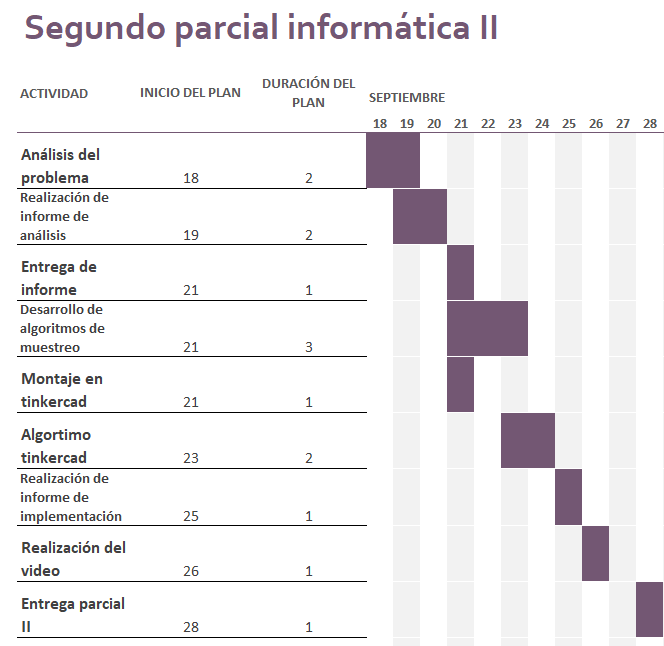
\includegraphics[width=10cm]{Esquema de tareas.PNG}
\centering
\caption{Esquema de tareas}
\label{fig:Esquema de tareas}
\end{figure}

\begin{figure}[h]
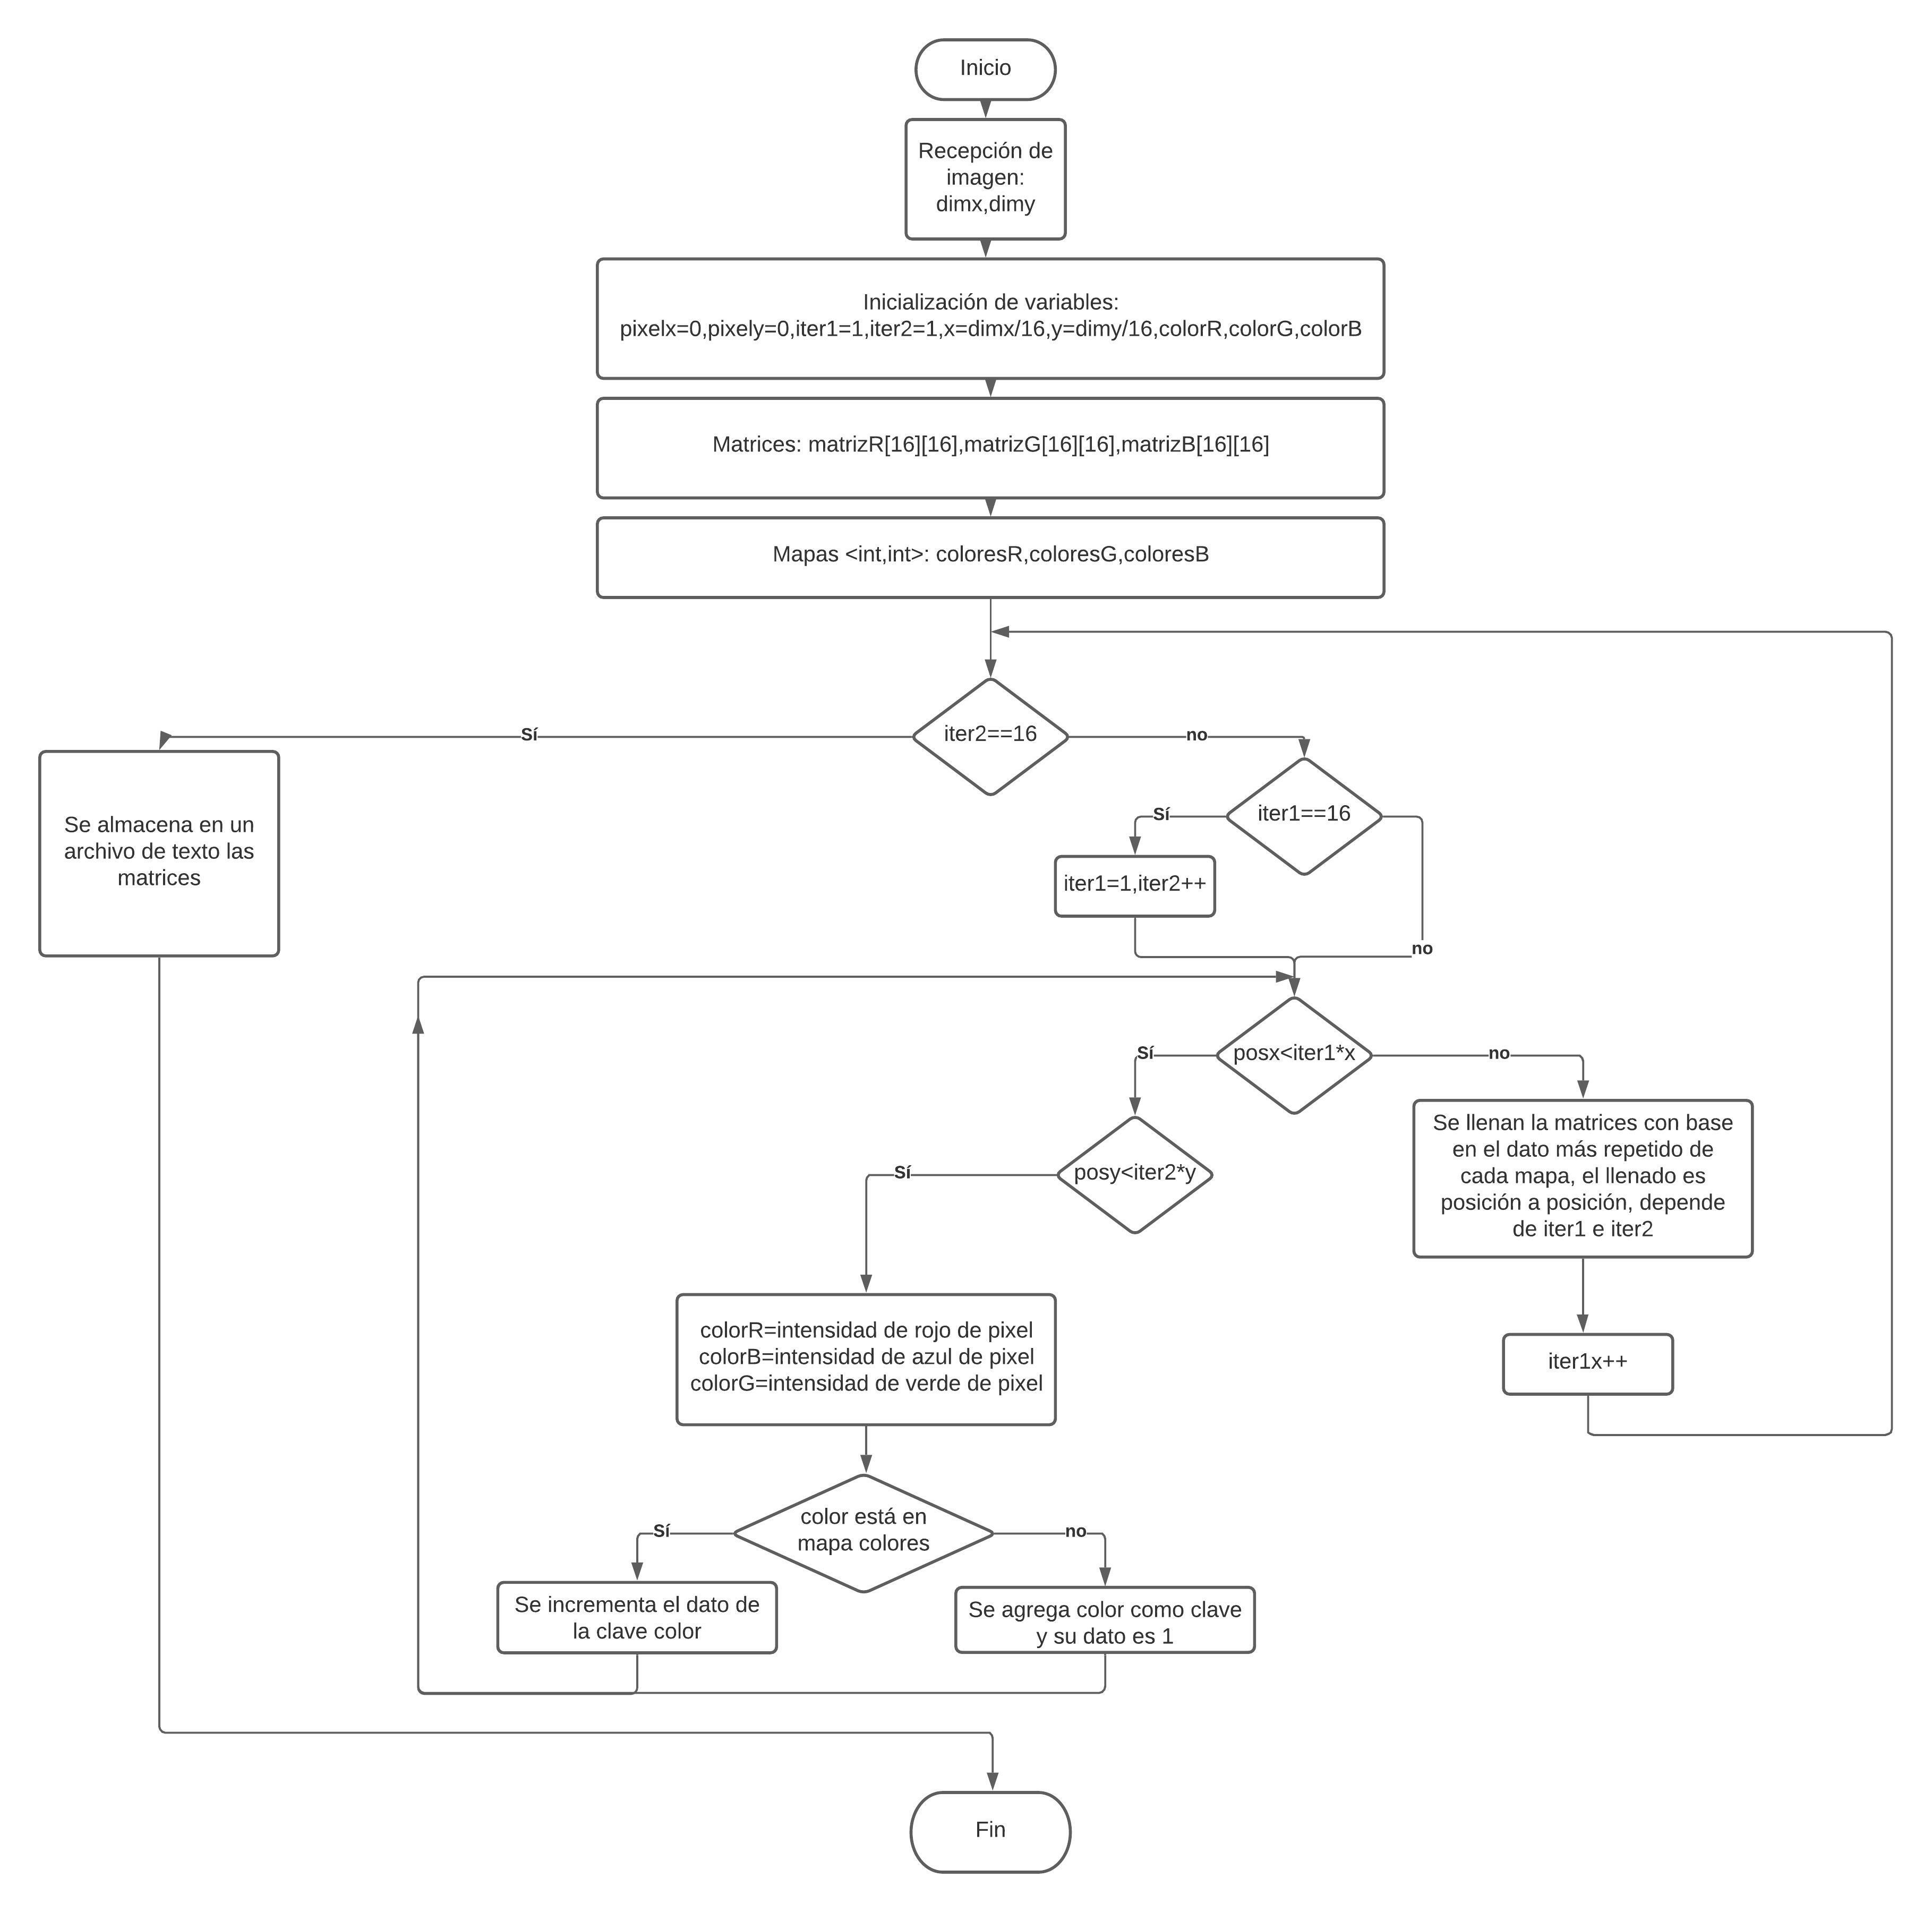
\includegraphics[width=12cm]{Algoritmo.jpeg}
\centering
\caption{Algoritmo}
\label{fig:Esquema de tareas}
\end{figure}

\end{document}
